% IMPORTANT: PLEASE USE XeLaTeX FOR TYPESETTING
\documentclass{beamer}

\usetheme{Darmstadt}%{default}
\usecolortheme{beaver}
\usepackage[T1]{fontenc} 
\usepackage[utf8]{inputenc}
\usepackage[french]{babel}
\usefonttheme{serif}
\usepackage{lmodern}
\usepackage{tcolorbox}
 % pour un pdf lisible à l'écran
 % il y a d'autres choix possibles 
\usepackage{pslatex}
% \usepackage{ctex, hyperref}
\usepackage{latexsym,amsmath,xcolor,multicol,booktabs,calligra}
\usepackage{graphicx,pstricks,listings,stackengine}
\usepackage{chemfig}
% meta-data
\title{Leçon : De la structure à la polarité d'une entité (Premiere générale)}
\subtitle{Élément imposé: Visualiser la géométrie d'une entité par utilisation de modèles moléculaires ou de logiciel de représentation moléculaire}

\author{Gabriel Le Doudic}
\institute{Préparation à l'agrégation de Rennes}
% \titlebackground{images/background}

\definecolor{aquamarine}{rgb}{0.5, 1.0, 0.83}
\definecolor{applegreen}{rgb}{0.55, 0.71, 0.0}	
\definecolor{cobalt}{rgb}{0.0, 0.28, 0.67}

\definecolor{definitionf}{RGB}{220,252,220}
\definecolor{definitionl}{RGB}{39,123,69}
\definecolor{definitiono}{RGB}{72,148,101}

\definecolor{propositionf}{RGB}{255,216,218}
\definecolor{propositionl}{RGB}{38,38,38}
\definecolor{propositiono}{RGB}{109,109,109}

\definecolor{theof}{RGB}{255,216,218}
\definecolor{theol}{RGB}{160,0,4}
\definecolor{theoo}{RGB}{221,65,100}

\definecolor{avertl}{RGB}{163,92,0}
\definecolor{averto}{RGB}{255,144,0}

\definecolor{histf}{RGB}{241,238,193}

\definecolor{metf}{RGB}{220,230,240}
\definecolor{metl}{RGB}{56,110,165}
\definecolor{meto}{RGB}{109,109,109}


\definecolor{remf}{RGB}{230,240,250}
\definecolor{remo}{RGB}{150,150,150}

\definecolor{exef}{RGB}{240,240,240}

\definecolor{protf}{RGB}{247,228,255}
\definecolor{protl}{RGB}{105,0,203}
\definecolor{proto}{RGB}{174,88,255}

\definecolor{grid}{RGB}{180,180,180}

\definecolor{titref}{RGB}{230,230,230}

\definecolor{vert}{RGB}{23,200,23}

\definecolor{violet}{RGB}{180,0,200}

\definecolor{copper}{RGB}{217, 144, 88}
%% CADRES

\newtcolorbox{defi}[1]{
	colback=applegreen!5!white,
  	colframe=applegreen!65!black,
	fonttitle=\bfseries,
  	title={#1}}
\newtcolorbox{Programme}[1]{
	colback=cobalt!5!white,
  	colframe=cobalt!65!black,
	fonttitle=\bfseries,
  	title={#1}}  
\newtcolorbox{Resultat}[1]{
	colback=theof,%!5!white,
	colframe=theoo!85!black,
  fonttitle=\bfseries,
	title={#1}} 
\usepackage{tikz}
\usetikzlibrary{matrix}
% document body
\begin{document}
\maketitle
% --------- Sommaire ---------
% \begin{frame}
%     \tableofcontents
% \end{frame}      
% ----------------------------

\begin{frame}{Bulletin officiel}
    \begin{figure}
        \centering
        \includegraphics[width=.7\textwidth]{Bo.png}
    \end{figure}
\end{frame}

\begin{frame}
    \tableofcontents
\end{frame}

\begin{frame}{Biblio}
    \begin{itemize}
        \item nathan 1ere 2019
        \item Belin 
        \item Hatier 2011 1ere 
    \end{itemize}
\end{frame}
\section{Schéma de Lewis}
\subsection{Doublets de Valence}

\begin{frame}
    \begin{figure}
        \centering
        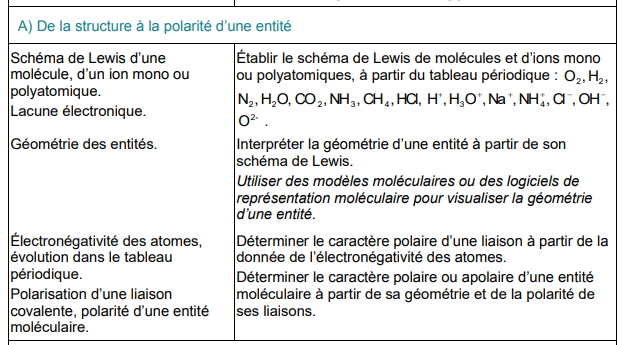
\includegraphics[width=.5\textwidth]{BO.png}
    \end{figure}
\end{frame}
\subsection{Construction d'un schéma de Lewis}
\subsection{Géométrie}

\begin{frame}
    \begin{itemize}
        \item     \url{https://www.ccdc.cam.ac.uk/}
        \item \url{http://www.crystallography.net/cod/index.php}
    \end{itemize}

\end{frame}
\section{Polarité d'une molécule}
\subsection{Notion d'électronégativité}
\subsection{Molécule polaire ou apolaire}
\end{document}